\documentclass[1p]{elsarticle_modified}
%\bibliographystyle{elsarticle-num}

%\usepackage[colorlinks]{hyperref}
%\usepackage{abbrmath_seonhwa} %\Abb, \Ascr, \Acal ,\Abf, \Afrak
\usepackage{amsfonts}
\usepackage{amssymb}
\usepackage{amsmath}
\usepackage{amsthm}
\usepackage{scalefnt}
\usepackage{amsbsy}
\usepackage{kotex}
\usepackage{caption}
\usepackage{subfig}
\usepackage{color}
\usepackage{graphicx}
\usepackage{xcolor} %% white, black, red, green, blue, cyan, magenta, yellow
\usepackage{float}
\usepackage{setspace}
\usepackage{hyperref}

\usepackage{tikz}
\usetikzlibrary{arrows}

\usepackage{multirow}
\usepackage{array} % fixed length table
\usepackage{hhline}

%%%%%%%%%%%%%%%%%%%%%
\makeatletter
\renewcommand*\env@matrix[1][\arraystretch]{%
	\edef\arraystretch{#1}%
	\hskip -\arraycolsep
	\let\@ifnextchar\new@ifnextchar
	\array{*\c@MaxMatrixCols c}}
\makeatother %https://tex.stackexchange.com/questions/14071/how-can-i-increase-the-line-spacing-in-a-matrix
%%%%%%%%%%%%%%%

\usepackage[normalem]{ulem}

\newcommand{\msout}[1]{\ifmmode\text{\sout{\ensuremath{#1}}}\else\sout{#1}\fi}
%SOURCE: \msout is \stkout macro in https://tex.stackexchange.com/questions/20609/strikeout-in-math-mode

\newcommand{\cancel}[1]{
	\ifmmode
	{\color{red}\msout{#1}}
	\else
	{\color{red}\sout{#1}}
	\fi
}

\newcommand{\add}[1]{
	{\color{blue}\uwave{#1}}
}

\newcommand{\replace}[2]{
	\ifmmode
	{\color{red}\msout{#1}}{\color{blue}\uwave{#2}}
	\else
	{\color{red}\sout{#1}}{\color{blue}\uwave{#2}}
	\fi
}

\newcommand{\Sol}{\mathcal{S}} %segment
\newcommand{\D}{D} %diagram
\newcommand{\A}{\mathcal{A}} %arc


%%%%%%%%%%%%%%%%%%%%%%%%%%%%%5 test

\def\sl{\operatorname{\textup{SL}}(2,\Cbb)}
\def\psl{\operatorname{\textup{PSL}}(2,\Cbb)}
\def\quan{\mkern 1mu \triangleright \mkern 1mu}

\theoremstyle{definition}
\newtheorem{thm}{Theorem}[section]
\newtheorem{prop}[thm]{Proposition}
\newtheorem{lem}[thm]{Lemma}
\newtheorem{ques}[thm]{Question}
\newtheorem{cor}[thm]{Corollary}
\newtheorem{defn}[thm]{Definition}
\newtheorem{exam}[thm]{Example}
\newtheorem{rmk}[thm]{Remark}
\newtheorem{alg}[thm]{Algorithm}

\newcommand{\I}{\sqrt{-1}}
\begin{document}

%\begin{frontmatter}
%
%\title{Boundary parabolic representations of knots up to 8 crossings}
%
%%% Group authors per affiliation:
%\author{Yunhi Cho} 
%\address{Department of Mathematics, University of Seoul, Seoul, Korea}
%\ead{yhcho@uos.ac.kr}
%
%
%\author{Seonhwa Kim} %\fnref{s_kim}}
%\address{Center for Geometry and Physics, Institute for Basic Science, Pohang, 37673, Korea}
%\ead{ryeona17@ibs.re.kr}
%
%\author{Hyuk Kim}
%\address{Department of Mathematical Sciences, Seoul National University, Seoul 08826, Korea}
%\ead{hyukkim@snu.ac.kr}
%
%\author{Seokbeom Yoon}
%\address{Department of Mathematical Sciences, Seoul National University, Seoul, 08826,  Korea}
%\ead{sbyoon15@snu.ac.kr}
%
%\begin{abstract}
%We find all boundary parabolic representation of knots up to 8 crossings.
%
%\end{abstract}
%\begin{keyword}
%    \MSC[2010] 57M25 
%\end{keyword}
%
%\end{frontmatter}

%\linenumbers
%\tableofcontents
%
\newcommand\colored[1]{\textcolor{white}{\rule[-0.35ex]{0.8em}{1.4ex}}\kern-0.8em\color{red} #1}%
%\newcommand\colored[1]{\textcolor{white}{ #1}\kern-2.17ex	\textcolor{white}{ #1}\kern-1.81ex	\textcolor{white}{ #1}\kern-2.15ex\color{red}#1	}

{\Large $\underline{10_{73}~(K10a_{3})}$}

\setlength{\tabcolsep}{10pt}
\renewcommand{\arraystretch}{1.6}
\vspace{1cm}\begin{tabular}{m{100pt}>{\centering\arraybackslash}m{274pt}}
\multirow{5}{120pt}{
	\centering
	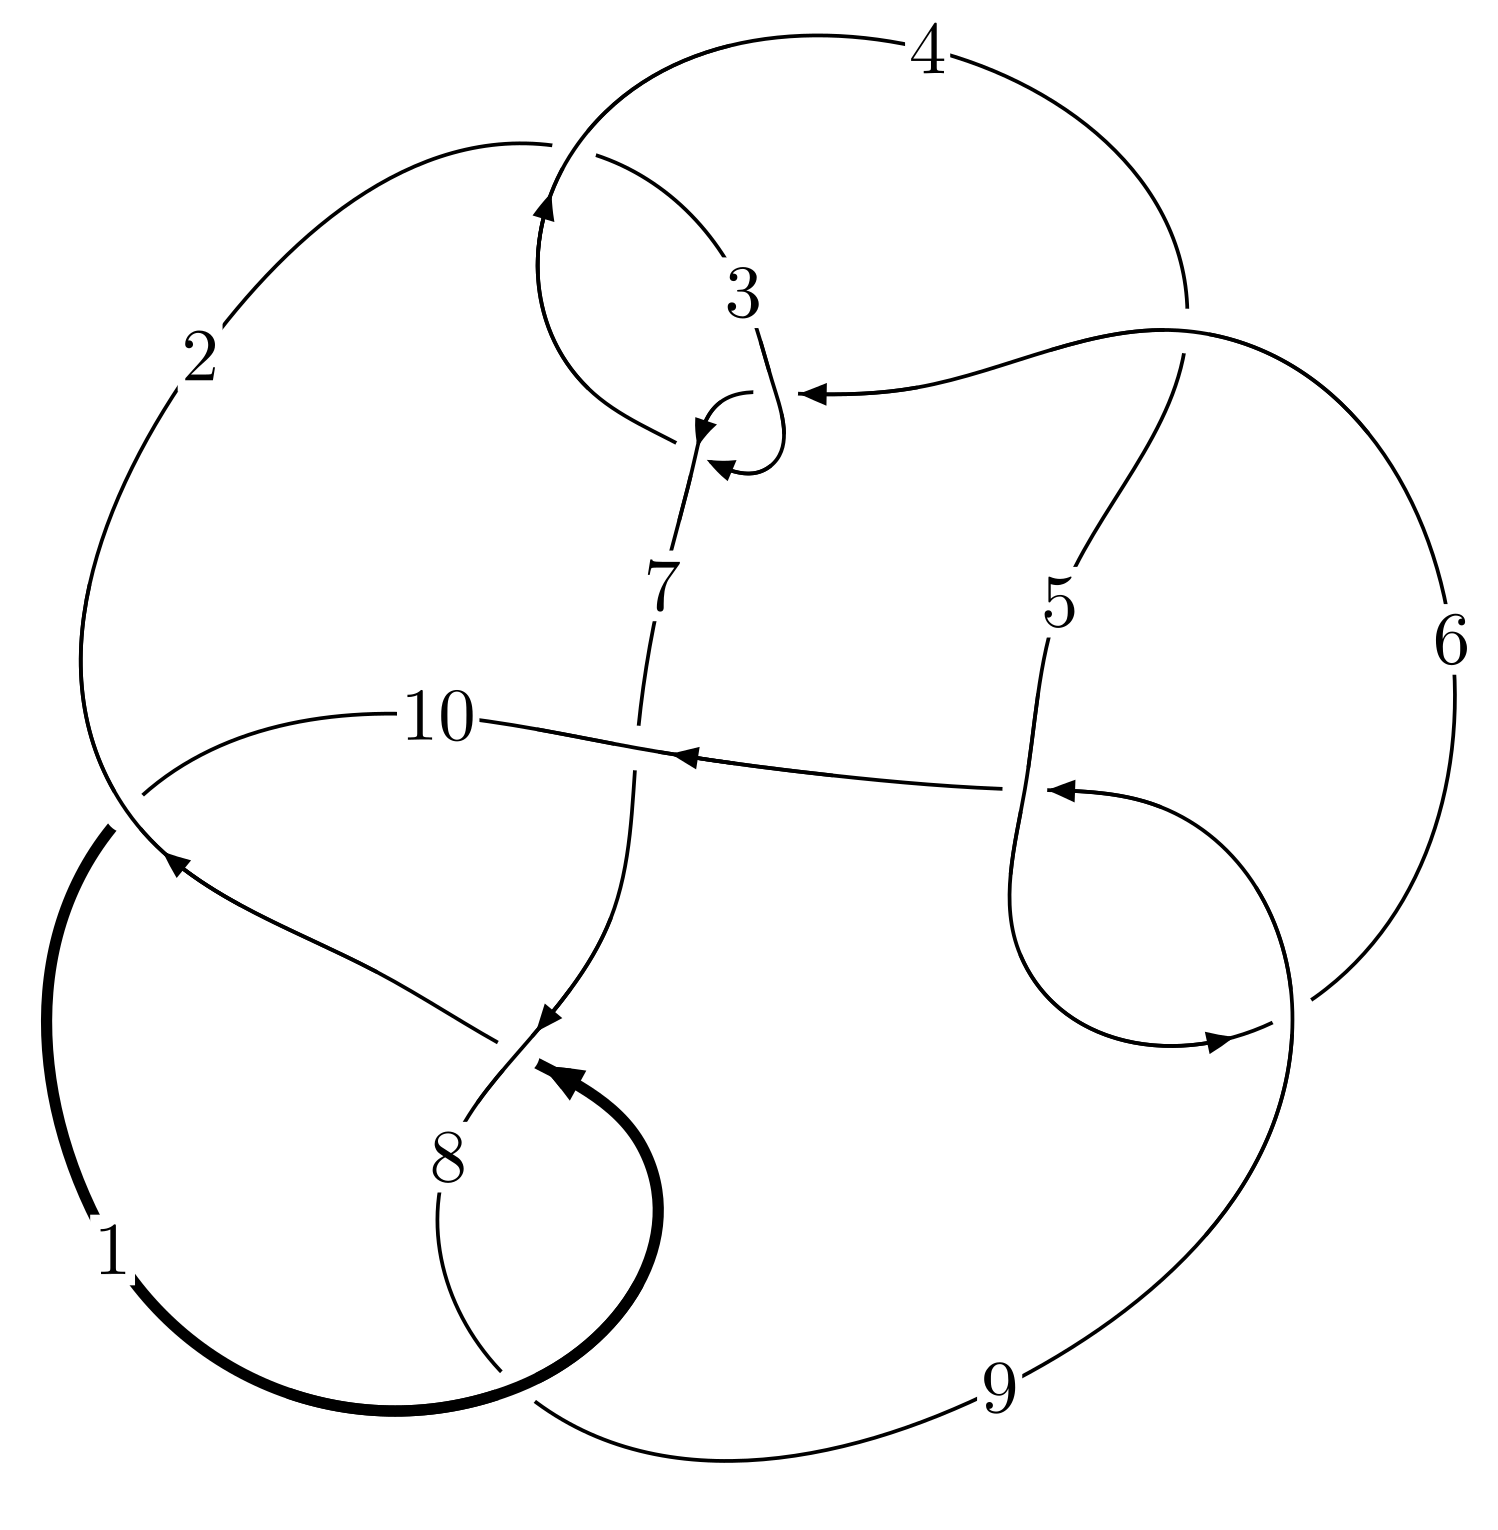
\includegraphics[width=112pt]{../../../GIT/diagram.site/Diagrams/png/157_10_73.png}\\
\ \ \ A knot diagram\footnotemark}&
\allowdisplaybreaks
\textbf{Linearized knot diagam} \\
\cline{2-2}
 &
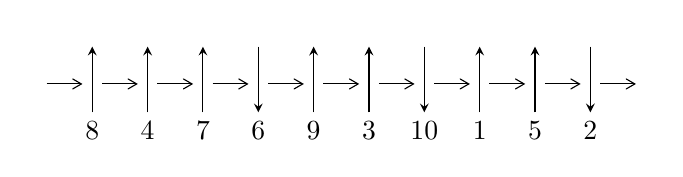
\begin{tikzpicture}[x=20pt, y=17pt]
	% nodes
	\node (C0) at (0, 0) {};
	\node (C1) at (1, 0) {};
	\node (C1U) at (1, +1) {};
	\node (C1D) at (1, -1) {8};

	\node (C2) at (2, 0) {};
	\node (C2U) at (2, +1) {};
	\node (C2D) at (2, -1) {4};

	\node (C3) at (3, 0) {};
	\node (C3U) at (3, +1) {};
	\node (C3D) at (3, -1) {7};

	\node (C4) at (4, 0) {};
	\node (C4U) at (4, +1) {};
	\node (C4D) at (4, -1) {6};

	\node (C5) at (5, 0) {};
	\node (C5U) at (5, +1) {};
	\node (C5D) at (5, -1) {9};

	\node (C6) at (6, 0) {};
	\node (C6U) at (6, +1) {};
	\node (C6D) at (6, -1) {3};

	\node (C7) at (7, 0) {};
	\node (C7U) at (7, +1) {};
	\node (C7D) at (7, -1) {10};

	\node (C8) at (8, 0) {};
	\node (C8U) at (8, +1) {};
	\node (C8D) at (8, -1) {1};

	\node (C9) at (9, 0) {};
	\node (C9U) at (9, +1) {};
	\node (C9D) at (9, -1) {5};

	\node (C10) at (10, 0) {};
	\node (C10U) at (10, +1) {};
	\node (C10D) at (10, -1) {2};
	\node (C11) at (11, 0) {};

	% arrows
	\draw[->,>={angle 60}]
	(C0) edge (C1) (C1) edge (C2) (C2) edge (C3) (C3) edge (C4) (C4) edge (C5) (C5) edge (C6) (C6) edge (C7) (C7) edge (C8) (C8) edge (C9) (C9) edge (C10) (C10) edge (C11) ;	\draw[->,>=stealth]
	(C1D) edge (C1U) (C2D) edge (C2U) (C3D) edge (C3U) (C4U) edge (C4D) (C5D) edge (C5U) (C6D) edge (C6U) (C7U) edge (C7D) (C8D) edge (C8U) (C9D) edge (C9U) (C10U) edge (C10D) ;
	\end{tikzpicture} \\
\hhline{~~} \\& 
\textbf{Solving Sequence} \\ \cline{2-2} 
 &
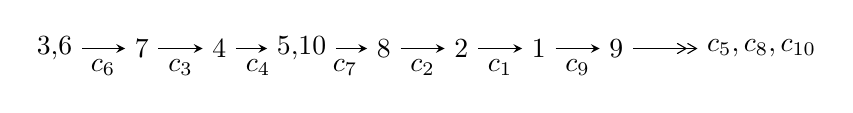
\begin{tikzpicture}[x=28pt, y=7pt]
	% node
	\node (A0) at (-1/8, 0) {3,6};
	\node (A1) at (1, 0) {7};
	\node (A2) at (2, 0) {4};
	\node (A3) at (49/16, 0) {5,10};
	\node (A4) at (33/8, 0) {8};
	\node (A5) at (41/8, 0) {2};
	\node (A6) at (49/8, 0) {1};
	\node (A7) at (57/8, 0) {9};
	\node (C1) at (1/2, -1) {$c_{6}$};
	\node (C2) at (3/2, -1) {$c_{3}$};
	\node (C3) at (5/2, -1) {$c_{4}$};
	\node (C4) at (29/8, -1) {$c_{7}$};
	\node (C5) at (37/8, -1) {$c_{2}$};
	\node (C6) at (45/8, -1) {$c_{1}$};
	\node (C7) at (53/8, -1) {$c_{9}$};
	\node (A8) at (9, 0) {$c_{5},c_{8},c_{10}$};

	% edge
	\draw[->,>=stealth]	
	(A0) edge (A1) (A1) edge (A2) (A2) edge (A3) (A3) edge (A4) (A4) edge (A5) (A5) edge (A6) (A6) edge (A7) ;
	\draw[->>,>={angle 60}]	
	(A7) edge (A8);
\end{tikzpicture} \\ 

\end{tabular} \\

\footnotetext{
The image of knot diagram is generated by the software ``\textbf{Draw programme}" developed by Andrew Bartholomew(\url{http://www.layer8.co.uk/maths/draw/index.htm\#Running-draw}), where we modified some parts for our purpose(\url{https://github.com/CATsTAILs/LinksPainter}).
}\phantom \\ \newline 
\centering \textbf{Ideals for irreducible components\footnotemark of $X_{\text{par}}$} 
 
\begin{align*}
I^u_{1}&=\langle 
- u^{42}- u^{41}+\cdots+u^2+b,\;-11 u^{42}-26 u^{41}+\cdots+2 a+15,\;u^{43}+3 u^{42}+\cdots-3 u-1\rangle \\
I^u_{2}&=\langle 
b,\;a^2- a+1,\;u-1\rangle \\
\\
\end{align*}
\raggedright * 2 irreducible components of $\dim_{\mathbb{C}}=0$, with total 45 representations.\\
\footnotetext{All coefficients of polynomials are rational numbers. But the coefficients are sometimes approximated in decimal forms when there is not enough margin.}
\newpage
\renewcommand{\arraystretch}{1}
\centering \section*{I. $I^u_{1}= \langle - u^{42}- u^{41}+\cdots+u^2+b,\;-11 u^{42}-26 u^{41}+\cdots+2 a+15,\;u^{43}+3 u^{42}+\cdots-3 u-1 \rangle$}
\flushleft \textbf{(i) Arc colorings}\\
\begin{tabular}{m{7pt} m{180pt} m{7pt} m{180pt} }
\flushright $a_{3}=$&$\begin{pmatrix}0\\u\end{pmatrix}$ \\
\flushright $a_{6}=$&$\begin{pmatrix}1\\0\end{pmatrix}$ \\
\flushright $a_{7}=$&$\begin{pmatrix}1\\- u^2\end{pmatrix}$ \\
\flushright $a_{4}=$&$\begin{pmatrix}u\\- u^3+u\end{pmatrix}$ \\
\flushright $a_{5}=$&$\begin{pmatrix}u^3\\- u^3+u\end{pmatrix}$ \\
\flushright $a_{10}=$&$\begin{pmatrix}\frac{11}{2} u^{42}+13 u^{41}+\cdots-13 u-\frac{15}{2}\\u^{42}+u^{41}+\cdots- u^3- u^2\end{pmatrix}$ \\
\flushright $a_{8}=$&$\begin{pmatrix}-\frac{1}{2} u^{42}- u^{41}+\cdots+u+\frac{1}{2}\\u^{11}-3 u^9-2 u^8+4 u^7+4 u^6- u^5-4 u^4- u^3+u\end{pmatrix}$ \\
\flushright $a_{2}=$&$\begin{pmatrix}- u^3\\u^5- u^3+u\end{pmatrix}$ \\
\flushright $a_{1}=$&$\begin{pmatrix}5 u^{42}+11 u^{41}+\cdots-11 u-6\\\frac{3}{2} u^{42}+3 u^{41}+\cdots-2 u-\frac{3}{2}\end{pmatrix}$ \\
\flushright $a_{9}=$&$\begin{pmatrix}\frac{11}{2} u^{42}+11 u^{41}+\cdots-11 u-\frac{13}{2}\\u^{41}+2 u^{40}+\cdots- u-1\end{pmatrix}$\\&\end{tabular}
\flushleft \textbf{(ii) Obstruction class $= -1$}\\~\\
\flushleft \textbf{(iii) Cusp Shapes $= -6 u^{42}-15 u^{41}+\cdots+19 u+13$}\\~\\
\newpage\renewcommand{\arraystretch}{1}
\flushleft \textbf{(iv) u-Polynomials at the component}\newline \\
\begin{tabular}{m{50pt}|m{274pt}}
Crossings & \hspace{64pt}u-Polynomials at each crossing \\
\hline $$\begin{aligned}c_{1},c_{8}\end{aligned}$$&$\begin{aligned}
&u^{43}+2 u^{42}+\cdots+4 u^2-1
\end{aligned}$\\
\hline $$\begin{aligned}c_{2}\end{aligned}$$&$\begin{aligned}
&u^{43}-23 u^{42}+\cdots+3 u-1
\end{aligned}$\\
\hline $$\begin{aligned}c_{3},c_{6}\end{aligned}$$&$\begin{aligned}
&u^{43}+3 u^{42}+\cdots-3 u-1
\end{aligned}$\\
\hline $$\begin{aligned}c_{4}\end{aligned}$$&$\begin{aligned}
&u^{43}+15 u^{42}+\cdots-136 u-16
\end{aligned}$\\
\hline $$\begin{aligned}c_{5},c_{9}\end{aligned}$$&$\begin{aligned}
&u^{43}- u^{42}+\cdots+8 u-4
\end{aligned}$\\
\hline $$\begin{aligned}c_{7}\end{aligned}$$&$\begin{aligned}
&u^{43}-2 u^{42}+\cdots+54 u-9
\end{aligned}$\\
\hline $$\begin{aligned}c_{10}\end{aligned}$$&$\begin{aligned}
&u^{43}+20 u^{42}+\cdots+8 u-1
\end{aligned}$\\
\hline
\end{tabular}\\~\\
\newpage\renewcommand{\arraystretch}{1}
\flushleft \textbf{(v) Riley Polynomials at the component}\newline \\
\begin{tabular}{m{50pt}|m{274pt}}
Crossings & \hspace{64pt}Riley Polynomials at each crossing \\
\hline $$\begin{aligned}c_{1},c_{8}\end{aligned}$$&$\begin{aligned}
&y^{43}+20 y^{42}+\cdots+8 y-1
\end{aligned}$\\
\hline $$\begin{aligned}c_{2}\end{aligned}$$&$\begin{aligned}
&y^{43}-3 y^{42}+\cdots+23 y-1
\end{aligned}$\\
\hline $$\begin{aligned}c_{3},c_{6}\end{aligned}$$&$\begin{aligned}
&y^{43}-23 y^{42}+\cdots+3 y-1
\end{aligned}$\\
\hline $$\begin{aligned}c_{4}\end{aligned}$$&$\begin{aligned}
&y^{43}+23 y^{42}+\cdots+4128 y-256
\end{aligned}$\\
\hline $$\begin{aligned}c_{5},c_{9}\end{aligned}$$&$\begin{aligned}
&y^{43}+15 y^{42}+\cdots-136 y-16
\end{aligned}$\\
\hline $$\begin{aligned}c_{7}\end{aligned}$$&$\begin{aligned}
&y^{43}-4 y^{42}+\cdots+2520 y-81
\end{aligned}$\\
\hline $$\begin{aligned}c_{10}\end{aligned}$$&$\begin{aligned}
&y^{43}+8 y^{42}+\cdots+140 y-1
\end{aligned}$\\
\hline
\end{tabular}\\~\\
\newpage\flushleft \textbf{(vi) Complex Volumes and Cusp Shapes}
$$\begin{array}{c|c|c}  
\text{Solutions to }I^u_{1}& \I (\text{vol} + \sqrt{-1}CS) & \text{Cusp shape}\\
 \hline 
\begin{aligned}
u &= -0.702205 + 0.692426 I \\
a &= -0.216763 + 1.063530 I \\
b &= -0.000164 - 0.427737 I\end{aligned}
 & -5.79250 + 1.33127 I & -3.13829 - 0.68119 I \\ \hline\begin{aligned}
u &= -0.702205 - 0.692426 I \\
a &= -0.216763 - 1.063530 I \\
b &= -0.000164 + 0.427737 I\end{aligned}
 & -5.79250 - 1.33127 I & -3.13829 + 0.68119 I \\ \hline\begin{aligned}
u &= -0.781262 + 0.586254 I \\
a &= \phantom{-}0.083513 - 0.751531 I \\
b &= -0.318284 + 0.078334 I\end{aligned}
 & -2.37041 - 2.31340 I & \phantom{-}1.61332 + 3.65794 I \\ \hline\begin{aligned}
u &= -0.781262 - 0.586254 I \\
a &= \phantom{-}0.083513 + 0.751531 I \\
b &= -0.318284 - 0.078334 I\end{aligned}
 & -2.37041 + 2.31340 I & \phantom{-}1.61332 - 3.65794 I \\ \hline\begin{aligned}
u &= \phantom{-}0.983429 + 0.401988 I \\
a &= -0.18299 + 1.51178 I \\
b &= \phantom{-}0.95580 - 1.21635 I\end{aligned}
 & \phantom{-}0.117899 + 0.694763 I & \phantom{-}2.77512 - 0.93635 I \\ \hline\begin{aligned}
u &= \phantom{-}0.983429 - 0.401988 I \\
a &= -0.18299 - 1.51178 I \\
b &= \phantom{-}0.95580 + 1.21635 I\end{aligned}
 & \phantom{-}0.117899 - 0.694763 I & \phantom{-}2.77512 + 0.93635 I \\ \hline\begin{aligned}
u &= -0.856054 + 0.662832 I \\
a &= -0.459912 + 0.582589 I \\
b &= \phantom{-}0.671689 - 0.315858 I\end{aligned}
 & -5.34910 - 6.48185 I & -1.72488 + 7.04551 I \\ \hline\begin{aligned}
u &= -0.856054 - 0.662832 I \\
a &= -0.459912 - 0.582589 I \\
b &= \phantom{-}0.671689 + 0.315858 I\end{aligned}
 & -5.34910 + 6.48185 I & -1.72488 - 7.04551 I \\ \hline\begin{aligned}
u &= -0.225042 + 0.862192 I \\
a &= -0.295884 - 0.330542 I \\
b &= \phantom{-}1.27608 - 1.18759 I\end{aligned}
 & -1.69061 + 8.49752 I & \phantom{-}0.86281 - 6.51033 I \\ \hline\begin{aligned}
u &= -0.225042 - 0.862192 I \\
a &= -0.295884 + 0.330542 I \\
b &= \phantom{-}1.27608 + 1.18759 I\end{aligned}
 & -1.69061 - 8.49752 I & \phantom{-}0.86281 + 6.51033 I\\
 \hline 
 \end{array}$$\newpage$$\begin{array}{c|c|c}  
\text{Solutions to }I^u_{1}& \I (\text{vol} + \sqrt{-1}CS) & \text{Cusp shape}\\
 \hline 
\begin{aligned}
u &= -0.344780 + 0.758252 I \\
a &= -0.130381 - 0.811333 I \\
b &= \phantom{-}0.921218 - 0.514197 I\end{aligned}
 & -4.05606 + 1.05891 I & -2.88403 - 0.52575 I \\ \hline\begin{aligned}
u &= -0.344780 - 0.758252 I \\
a &= -0.130381 + 0.811333 I \\
b &= \phantom{-}0.921218 + 0.514197 I\end{aligned}
 & -4.05606 - 1.05891 I & -2.88403 + 0.52575 I \\ \hline\begin{aligned}
u &= -0.199953 + 0.800457 I \\
a &= \phantom{-}0.051467 + 0.372242 I \\
b &= -0.93072 + 1.17107 I\end{aligned}
 & \phantom{-}0.47003 + 3.49797 I & \phantom{-}3.95877 - 2.64358 I \\ \hline\begin{aligned}
u &= -0.199953 - 0.800457 I \\
a &= \phantom{-}0.051467 - 0.372242 I \\
b &= -0.93072 - 1.17107 I\end{aligned}
 & \phantom{-}0.47003 - 3.49797 I & \phantom{-}3.95877 + 2.64358 I \\ \hline\begin{aligned}
u &= \phantom{-}1.178400 + 0.107020 I \\
a &= \phantom{-}0.396216 - 0.024715 I \\
b &= -0.090847 - 0.484893 I\end{aligned}
 & \phantom{-}0.86535 + 1.34877 I & \phantom{-}0.663414 + 0.523198 I \\ \hline\begin{aligned}
u &= \phantom{-}1.178400 - 0.107020 I \\
a &= \phantom{-}0.396216 + 0.024715 I \\
b &= -0.090847 + 0.484893 I\end{aligned}
 & \phantom{-}0.86535 - 1.34877 I & \phantom{-}0.663414 - 0.523198 I \\ \hline\begin{aligned}
u &= -1.113040 + 0.411275 I \\
a &= -1.45881 + 1.05016 I \\
b &= -0.432177 - 1.242820 I\end{aligned}
 & \phantom{-}3.14686 - 0.23394 I & \phantom{-}6.25545 + 1.76917 I \\ \hline\begin{aligned}
u &= -1.113040 - 0.411275 I \\
a &= -1.45881 - 1.05016 I \\
b &= -0.432177 + 1.242820 I\end{aligned}
 & \phantom{-}3.14686 + 0.23394 I & \phantom{-}6.25545 - 1.76917 I \\ \hline\begin{aligned}
u &= \phantom{-}1.140070 + 0.437496 I \\
a &= -0.80318 - 1.92969 I \\
b &= -0.35123 + 1.92571 I\end{aligned}
 & \phantom{-}4.51030 + 2.45703 I & \phantom{-}9.07720 - 1.39524 I \\ \hline\begin{aligned}
u &= \phantom{-}1.140070 - 0.437496 I \\
a &= -0.80318 + 1.92969 I \\
b &= -0.35123 - 1.92571 I\end{aligned}
 & \phantom{-}4.51030 - 2.45703 I & \phantom{-}9.07720 + 1.39524 I\\
 \hline 
 \end{array}$$\newpage$$\begin{array}{c|c|c}  
\text{Solutions to }I^u_{1}& \I (\text{vol} + \sqrt{-1}CS) & \text{Cusp shape}\\
 \hline 
\begin{aligned}
u &= \phantom{-}1.126240 + 0.485857 I \\
a &= \phantom{-}0.62977 + 2.31079 I \\
b &= \phantom{-}0.62085 - 2.17017 I\end{aligned}
 & \phantom{-}2.59778 + 7.42216 I & \phantom{-}5.67783 - 6.16302 I \\ \hline\begin{aligned}
u &= \phantom{-}1.126240 - 0.485857 I \\
a &= \phantom{-}0.62977 - 2.31079 I \\
b &= \phantom{-}0.62085 + 2.17017 I\end{aligned}
 & \phantom{-}2.59778 - 7.42216 I & \phantom{-}5.67783 + 6.16302 I \\ \hline\begin{aligned}
u &= -1.139980 + 0.455119 I \\
a &= \phantom{-}1.12604 - 1.46501 I \\
b &= \phantom{-}0.68367 + 1.40137 I\end{aligned}
 & \phantom{-}4.38701 - 5.48645 I & \phantom{-}8.10083 + 6.46210 I \\ \hline\begin{aligned}
u &= -1.139980 - 0.455119 I \\
a &= \phantom{-}1.12604 + 1.46501 I \\
b &= \phantom{-}0.68367 - 1.40137 I\end{aligned}
 & \phantom{-}4.38701 + 5.48645 I & \phantom{-}8.10083 - 6.46210 I \\ \hline\begin{aligned}
u &= \phantom{-}0.769344\phantom{ +0.000000I} \\
a &= -0.716816\phantom{ +0.000000I} \\
b &= \phantom{-}0.736269\phantom{ +0.000000I}\end{aligned}
 & \phantom{-}1.12210\phantom{ +0.000000I} & \phantom{-}9.24310\phantom{ +0.000000I} \\ \hline\begin{aligned}
u &= -1.116400 + 0.556388 I \\
a &= -0.04192 + 1.41433 I \\
b &= -1.30408 - 1.10564 I\end{aligned}
 & -1.77735 - 6.01104 I & \phantom{-0.000000 -}0. + 4.92263 I \\ \hline\begin{aligned}
u &= -1.116400 - 0.556388 I \\
a &= -0.04192 - 1.41433 I \\
b &= -1.30408 + 1.10564 I\end{aligned}
 & -1.77735 + 6.01104 I & \phantom{-0.000000 } 0. - 4.92263 I \\ \hline\begin{aligned}
u &= \phantom{-}1.207770 + 0.337329 I \\
a &= -1.27016 - 1.08338 I \\
b &= \phantom{-}0.27337 + 1.44443 I\end{aligned}
 & \phantom{-}4.74199 + 0.21154 I & \phantom{-}9.28481 + 0. I\phantom{ +0.000000I} \\ \hline\begin{aligned}
u &= \phantom{-}1.207770 - 0.337329 I \\
a &= -1.27016 + 1.08338 I \\
b &= \phantom{-}0.27337 - 1.44443 I\end{aligned}
 & \phantom{-}4.74199 - 0.21154 I & \phantom{-}9.28481 + 0. I\phantom{ +0.000000I} \\ \hline\begin{aligned}
u &= \phantom{-}0.596984 + 0.406248 I \\
a &= \phantom{-}1.37593 - 0.78349 I \\
b &= -1.384640 - 0.071781 I\end{aligned}
 & -1.01538 + 2.84865 I & \phantom{-}1.39768 - 5.43636 I\\
 \hline 
 \end{array}$$\newpage$$\begin{array}{c|c|c}  
\text{Solutions to }I^u_{1}& \I (\text{vol} + \sqrt{-1}CS) & \text{Cusp shape}\\
 \hline 
\begin{aligned}
u &= \phantom{-}0.596984 - 0.406248 I \\
a &= \phantom{-}1.37593 + 0.78349 I \\
b &= -1.384640 + 0.071781 I\end{aligned}
 & -1.01538 - 2.84865 I & \phantom{-}1.39768 + 5.43636 I \\ \hline\begin{aligned}
u &= \phantom{-}1.253070 + 0.301863 I \\
a &= \phantom{-}1.51757 + 0.68122 I \\
b &= -0.561583 - 1.231910 I\end{aligned}
 & \phantom{-}3.01994 - 4.67918 I & \phantom{-0.000000 -}0. + 5.37573 I \\ \hline\begin{aligned}
u &= \phantom{-}1.253070 - 0.301863 I \\
a &= \phantom{-}1.51757 - 0.68122 I \\
b &= -0.561583 + 1.231910 I\end{aligned}
 & \phantom{-}3.01994 + 4.67918 I & \phantom{-0.000000 } 0. - 5.37573 I \\ \hline\begin{aligned}
u &= -1.177230 + 0.535254 I \\
a &= \phantom{-}0.33951 - 2.06230 I \\
b &= \phantom{-}1.28426 + 1.59104 I\end{aligned}
 & \phantom{-}3.34693 - 8.44363 I & \phantom{-0.000000 } 0 \\ \hline\begin{aligned}
u &= -1.177230 - 0.535254 I \\
a &= \phantom{-}0.33951 + 2.06230 I \\
b &= \phantom{-}1.28426 - 1.59104 I\end{aligned}
 & \phantom{-}3.34693 + 8.44363 I & \phantom{-0.000000 } 0 \\ \hline\begin{aligned}
u &= -0.674002 + 0.118500 I \\
a &= -0.26643 - 1.82830 I \\
b &= -0.006255 - 0.381927 I\end{aligned}
 & \phantom{-}0.77235 - 2.35753 I & -0.15632 + 5.03988 I \\ \hline\begin{aligned}
u &= -0.674002 - 0.118500 I \\
a &= -0.26643 + 1.82830 I \\
b &= -0.006255 + 0.381927 I\end{aligned}
 & \phantom{-}0.77235 + 2.35753 I & -0.15632 - 5.03988 I \\ \hline\begin{aligned}
u &= -1.191540 + 0.559537 I \\
a &= -0.06666 + 2.26638 I \\
b &= -1.51037 - 1.66131 I\end{aligned}
 & \phantom{-}1.20075 - 13.70690 I & \phantom{-0.000000 } 0 \\ \hline\begin{aligned}
u &= -1.191540 - 0.559537 I \\
a &= -0.06666 - 2.26638 I \\
b &= -1.51037 + 1.66131 I\end{aligned}
 & \phantom{-}1.20075 + 13.70690 I & \phantom{-0.000000 } 0 \\ \hline\begin{aligned}
u &= -0.025551 + 0.621606 I \\
a &= -0.721932 + 0.454368 I \\
b &= \phantom{-}0.017381 + 1.186670 I\end{aligned}
 & \phantom{-}1.39154 + 1.44262 I & \phantom{-}5.16219 - 3.23191 I\\
 \hline 
 \end{array}$$\newpage$$\begin{array}{c|c|c}  
\text{Solutions to }I^u_{1}& \I (\text{vol} + \sqrt{-1}CS) & \text{Cusp shape}\\
 \hline 
\begin{aligned}
u &= -0.025551 - 0.621606 I \\
a &= -0.721932 - 0.454368 I \\
b &= \phantom{-}0.017381 - 1.186670 I\end{aligned}
 & \phantom{-}1.39154 - 1.44262 I & \phantom{-}5.16219 + 3.23191 I \\ \hline\begin{aligned}
u &= \phantom{-}0.176403 + 0.591173 I \\
a &= \phantom{-}1.253380 - 0.348319 I \\
b &= -0.682100 - 1.225820 I\end{aligned}
 & -0.03125 - 3.16118 I & \phantom{-}2.63487 + 2.30647 I \\ \hline\begin{aligned}
u &= \phantom{-}0.176403 - 0.591173 I \\
a &= \phantom{-}1.253380 + 0.348319 I \\
b &= -0.682100 + 1.225820 I\end{aligned}
 & -0.03125 + 3.16118 I & \phantom{-}2.63487 - 2.30647 I\\
 \hline 
 \end{array}$$\newpage\newpage\renewcommand{\arraystretch}{1}
\centering \section*{II. $I^u_{2}= \langle b,\;a^2- a+1,\;u-1 \rangle$}
\flushleft \textbf{(i) Arc colorings}\\
\begin{tabular}{m{7pt} m{180pt} m{7pt} m{180pt} }
\flushright $a_{3}=$&$\begin{pmatrix}0\\1\end{pmatrix}$ \\
\flushright $a_{6}=$&$\begin{pmatrix}1\\0\end{pmatrix}$ \\
\flushright $a_{7}=$&$\begin{pmatrix}1\\-1\end{pmatrix}$ \\
\flushright $a_{4}=$&$\begin{pmatrix}1\\0\end{pmatrix}$ \\
\flushright $a_{5}=$&$\begin{pmatrix}1\\0\end{pmatrix}$ \\
\flushright $a_{10}=$&$\begin{pmatrix}a\\0\end{pmatrix}$ \\
\flushright $a_{8}=$&$\begin{pmatrix}a\\-1\end{pmatrix}$ \\
\flushright $a_{2}=$&$\begin{pmatrix}-1\\1\end{pmatrix}$ \\
\flushright $a_{1}=$&$\begin{pmatrix}0\\a\end{pmatrix}$ \\
\flushright $a_{9}=$&$\begin{pmatrix}a\\0\end{pmatrix}$\\&\end{tabular}
\flushleft \textbf{(ii) Obstruction class $= 1$}\\~\\
\flushleft \textbf{(iii) Cusp Shapes $= 4 a+7$}\\~\\
\newpage\renewcommand{\arraystretch}{1}
\flushleft \textbf{(iv) u-Polynomials at the component}\newline \\
\begin{tabular}{m{50pt}|m{274pt}}
Crossings & \hspace{64pt}u-Polynomials at each crossing \\
\hline $$\begin{aligned}c_{1},c_{7},c_{10}\end{aligned}$$&$\begin{aligned}
&u^2- u+1
\end{aligned}$\\
\hline $$\begin{aligned}c_{2},c_{3}\end{aligned}$$&$\begin{aligned}
&(u+1)^2
\end{aligned}$\\
\hline $$\begin{aligned}c_{4},c_{5},c_{9}\end{aligned}$$&$\begin{aligned}
&u^2
\end{aligned}$\\
\hline $$\begin{aligned}c_{6}\end{aligned}$$&$\begin{aligned}
&(u-1)^2
\end{aligned}$\\
\hline $$\begin{aligned}c_{8}\end{aligned}$$&$\begin{aligned}
&u^2+u+1
\end{aligned}$\\
\hline
\end{tabular}\\~\\
\newpage\renewcommand{\arraystretch}{1}
\flushleft \textbf{(v) Riley Polynomials at the component}\newline \\
\begin{tabular}{m{50pt}|m{274pt}}
Crossings & \hspace{64pt}Riley Polynomials at each crossing \\
\hline $$\begin{aligned}c_{1},c_{7},c_{8}\\c_{10}\end{aligned}$$&$\begin{aligned}
&y^2+y+1
\end{aligned}$\\
\hline $$\begin{aligned}c_{2},c_{3},c_{6}\end{aligned}$$&$\begin{aligned}
&(y-1)^2
\end{aligned}$\\
\hline $$\begin{aligned}c_{4},c_{5},c_{9}\end{aligned}$$&$\begin{aligned}
&y^2
\end{aligned}$\\
\hline
\end{tabular}\\~\\
\newpage\flushleft \textbf{(vi) Complex Volumes and Cusp Shapes}
$$\begin{array}{c|c|c}  
\text{Solutions to }I^u_{2}& \I (\text{vol} + \sqrt{-1}CS) & \text{Cusp shape}\\
 \hline 
\begin{aligned}
u &= \phantom{-}1.00000\phantom{ +0.000000I} \\
a &= \phantom{-}0.500000 + 0.866025 I \\
b &= \phantom{-0.000000 } 0\end{aligned}
 & \phantom{-}1.64493 - 2.02988 I & \phantom{-}9.00000 + 3.46410 I \\ \hline\begin{aligned}
u &= \phantom{-}1.00000\phantom{ +0.000000I} \\
a &= \phantom{-}0.500000 - 0.866025 I \\
b &= \phantom{-0.000000 } 0\end{aligned}
 & \phantom{-}1.64493 + 2.02988 I & \phantom{-}9.00000 - 3.46410 I\\
 \hline 
 \end{array}$$\newpage
\newpage\renewcommand{\arraystretch}{1}
\centering \section*{ III. u-Polynomials}
\begin{tabular}{m{50pt}|m{274pt}}
Crossings & \hspace{64pt}u-Polynomials at each crossing \\
\hline $$\begin{aligned}c_{1}\end{aligned}$$&$\begin{aligned}
&(u^2- u+1)(u^{43}+2 u^{42}+\cdots+4 u^2-1)
\end{aligned}$\\
\hline $$\begin{aligned}c_{2}\end{aligned}$$&$\begin{aligned}
&((u+1)^2)(u^{43}-23 u^{42}+\cdots+3 u-1)
\end{aligned}$\\
\hline $$\begin{aligned}c_{3}\end{aligned}$$&$\begin{aligned}
&((u+1)^2)(u^{43}+3 u^{42}+\cdots-3 u-1)
\end{aligned}$\\
\hline $$\begin{aligned}c_{4}\end{aligned}$$&$\begin{aligned}
&u^2(u^{43}+15 u^{42}+\cdots-136 u-16)
\end{aligned}$\\
\hline $$\begin{aligned}c_{5},c_{9}\end{aligned}$$&$\begin{aligned}
&u^2(u^{43}- u^{42}+\cdots+8 u-4)
\end{aligned}$\\
\hline $$\begin{aligned}c_{6}\end{aligned}$$&$\begin{aligned}
&((u-1)^2)(u^{43}+3 u^{42}+\cdots-3 u-1)
\end{aligned}$\\
\hline $$\begin{aligned}c_{7}\end{aligned}$$&$\begin{aligned}
&(u^2- u+1)(u^{43}-2 u^{42}+\cdots+54 u-9)
\end{aligned}$\\
\hline $$\begin{aligned}c_{8}\end{aligned}$$&$\begin{aligned}
&(u^2+u+1)(u^{43}+2 u^{42}+\cdots+4 u^2-1)
\end{aligned}$\\
\hline $$\begin{aligned}c_{10}\end{aligned}$$&$\begin{aligned}
&(u^2- u+1)(u^{43}+20 u^{42}+\cdots+8 u-1)
\end{aligned}$\\
\hline
\end{tabular}\newpage\renewcommand{\arraystretch}{1}
\centering \section*{ IV. Riley Polynomials}
\begin{tabular}{m{50pt}|m{274pt}}
Crossings & \hspace{64pt}Riley Polynomials at each crossing \\
\hline $$\begin{aligned}c_{1},c_{8}\end{aligned}$$&$\begin{aligned}
&(y^2+y+1)(y^{43}+20 y^{42}+\cdots+8 y-1)
\end{aligned}$\\
\hline $$\begin{aligned}c_{2}\end{aligned}$$&$\begin{aligned}
&((y-1)^2)(y^{43}-3 y^{42}+\cdots+23 y-1)
\end{aligned}$\\
\hline $$\begin{aligned}c_{3},c_{6}\end{aligned}$$&$\begin{aligned}
&((y-1)^2)(y^{43}-23 y^{42}+\cdots+3 y-1)
\end{aligned}$\\
\hline $$\begin{aligned}c_{4}\end{aligned}$$&$\begin{aligned}
&y^2(y^{43}+23 y^{42}+\cdots+4128 y-256)
\end{aligned}$\\
\hline $$\begin{aligned}c_{5},c_{9}\end{aligned}$$&$\begin{aligned}
&y^2(y^{43}+15 y^{42}+\cdots-136 y-16)
\end{aligned}$\\
\hline $$\begin{aligned}c_{7}\end{aligned}$$&$\begin{aligned}
&(y^2+y+1)(y^{43}-4 y^{42}+\cdots+2520 y-81)
\end{aligned}$\\
\hline $$\begin{aligned}c_{10}\end{aligned}$$&$\begin{aligned}
&(y^2+y+1)(y^{43}+8 y^{42}+\cdots+140 y-1)
\end{aligned}$\\
\hline
\end{tabular}
\vskip 2pc
\end{document}